\chapter{Tools}


\includegraphics{../images/school-tools-3596680_1920.jpg}

We can reduce our Mean Time To Deploy (MTTD)
by using tools to prepare and generate our machine images
programatically, and with scripting languages such as HCL, which
Terraform
is based on. In this section we examine these tools in greater depth.

single: MTTD
single: Terraform

\begin{figure}
   \centering
   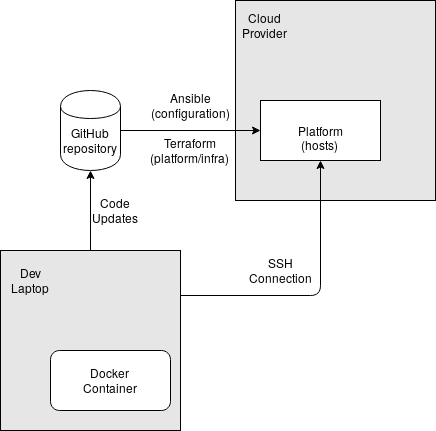
\includegraphics{../images/infra_flow.png}
   \caption{The pipeline flow.}
\end{figure}

Consider the following diagram {myFig4} as we discuss the tools we'll
use to implement our infrastructure as code and associated
configurations in the cloud provider network.

\section{Packer}

\justify
Using Hashicorp Packer is a great way to nail down the contents of a
machine image before we bring up an instance. Download Packer from the
Hashicorp web site in preparation for the following steps. 
We will focus on creating images for our cloud provider from the
command line. Bear in mind it is also possible to use Terraform to
manage the creation of Packer generated machine images. Generating
machine images on the fly using Terraform would increase our degree of
ephepmerality and immutability.

\subsection{Packer Example Configuration for AWS}

Here is an example of how to set up a JSON file to build a Packer image
in AWS. Save the contents of this file into
`packer/aws-debian-host.json`:

\justify
\begin{mybox}{\thetcbcounter: aws-debian-host.json}
	\lstinputlisting{code/aws-debian-host.json}
\end{mybox}

\subsection{Packer Example Configuration for GCP}

\justify
Here is an example of how to set up a JSON file to build a Packer image
in Google Compute. Save the contents of this file into
`packer/gcp-debian-host.json`:

\justify
\begin{mybox}{\thetcbcounter: gcp-debian-host.json}
	\lstinputlisting{code/gcp-debian-host.json}
\end{mybox}


\subsection{Validating Packer JSON Files}

\justify
Once the JSON files are created and saved in the packer directory, we
can use the packer tool to validate them. Type
packer validate \textless{}filename\textgreater{} to validate each new
JSON file. This gives you a chance to find and fix any errors before the
next step, the build phase.

\justify
Note that your validation commands may fail if the cloud provider
credentials have not been configured at this point.

\subsection{Building Images with Packer}

\justify
Finally, we are ready to build our new images. Try typing
packer build \textless{}filename\textgreater{} to create the image. You
should see output similar to the following, but with a unique AMI ID.

\begin{mybox}{\thetcbcounter: packer build}
Build 'amazon-ebs' finished.

==> Builds finished. The artifacts of successful builds are:
--> amazon-ebs: AMIs were created:
    us-west-2: ami-0e9e6427509a9d0b5
\end{mybox}

\justify
The AMI ID "ami-0e9e6427509a9d0b5" is now a usable image that we can
include in our Terraform builds.

\subsection{Removing Packer Images from Cloud Provider}

\justify
You may want to remove the images from AWS/GCP since storing them incurs
additional cost, whether they are in use or not.

\justify
To remove stale machine images from AWS, you may try a tool such as
aws-amicleaner, which is available to be installed via Python/pip as well as from the
GitHub repository for the project.

\jusitfy
Another AWS specfic tool is "lambda-packerjanitor" from Trusworks.

\section{Terraform}
\justify
Terraform, created by Hashicorp in 2014, is a tool for building, changing, and versioning 
infrastructure safely and efficiently . Install the latest version of Terraform
in preparation for the activities that follow.

\justify
Consider the relevant Terraform files that we will include in our
projects.

\begin{figure}[!htb]
	
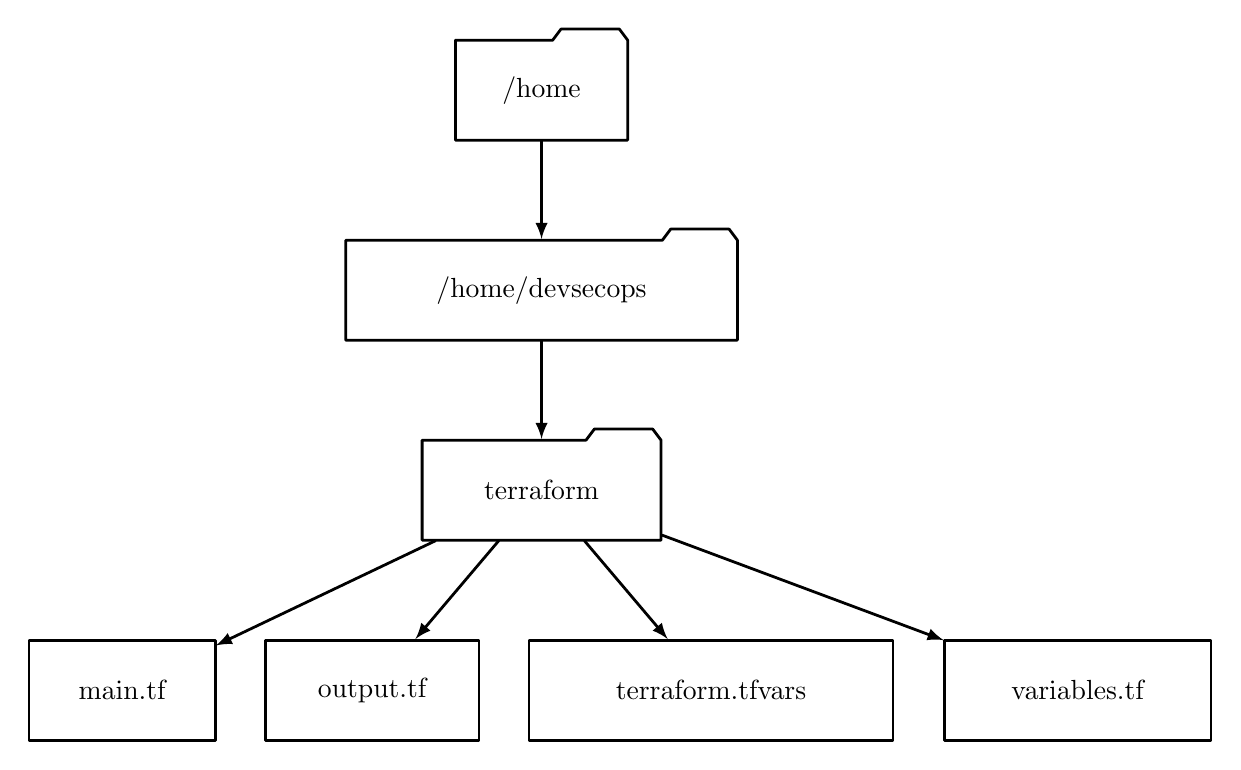
\begin{tikzpicture}[>=latex,line join=bevel,]
  \pgfsetlinewidth{1bp}
%%
\pgfsetcolor{black}
  % Edge: home -> devsecops
  \draw [->] (184.5bp,215.83bp) .. controls (184.5bp,208.13bp) and (184.5bp,198.97bp)  .. (184.5bp,180.41bp);
  % Edge: devsecops -> aws
  \draw [->] (184.5bp,143.83bp) .. controls (184.5bp,136.13bp) and (184.5bp,126.97bp)  .. (184.5bp,108.41bp);
  % Edge: aws -> main
  \draw [->] (146.4bp,71.831bp) .. controls (125.07bp,61.661bp) and (98.412bp,48.951bp)  .. (67.217bp,34.077bp);
  % Edge: aws -> out
  \draw [->] (169.11bp,71.831bp) .. controls (162.01bp,63.454bp) and (153.45bp,53.353bp)  .. (139.1bp,36.413bp);
  % Edge: aws -> tfvars
  \draw [->] (199.89bp,71.831bp) .. controls (206.99bp,63.454bp) and (215.55bp,53.353bp)  .. (229.9bp,36.413bp);
  % Edge: aws -> var
  \draw [->] (227.81bp,73.842bp) .. controls (254.87bp,63.747bp) and (290.05bp,50.625bp)  .. (329.25bp,36.001bp);
  % Node: home
\begin{scope}
  \definecolor{strokecol}{rgb}{0.0,0.0,0.0};
  \pgfsetstrokecolor{strokecol}
  \draw (215.5bp,252.0bp) -- (212.5bp,256.0bp) -- (191.5bp,256.0bp) -- (188.5bp,252.0bp) -- (153.5bp,252.0bp) -- (153.5bp,216.0bp) -- (215.5bp,216.0bp) -- cycle;
  \draw (184.5bp,234.0bp) node {/home};
\end{scope}
  % Node: devsecops
\begin{scope}
  \definecolor{strokecol}{rgb}{0.0,0.0,0.0};
  \pgfsetstrokecolor{strokecol}
  \draw (255.0bp,180.0bp) -- (252.0bp,184.0bp) -- (231.0bp,184.0bp) -- (228.0bp,180.0bp) -- (114.0bp,180.0bp) -- (114.0bp,144.0bp) -- (255.0bp,144.0bp) -- cycle;
  \draw (184.5bp,162.0bp) node {/home/devsecops};
\end{scope}
  % Node: aws
\begin{scope}
  \definecolor{strokecol}{rgb}{0.0,0.0,0.0};
  \pgfsetstrokecolor{strokecol}
  \draw (227.5bp,108.0bp) -- (224.5bp,112.0bp) -- (203.5bp,112.0bp) -- (200.5bp,108.0bp) -- (141.5bp,108.0bp) -- (141.5bp,72.0bp) -- (227.5bp,72.0bp) -- cycle;
  \draw (184.5bp,90.0bp) node {terraform};
\end{scope}
  % Node: main
\begin{scope}
  \definecolor{strokecol}{rgb}{0.0,0.0,0.0};
  \pgfsetstrokecolor{strokecol}
  \draw (67.0bp,36.0bp) -- (0.0bp,36.0bp) -- (0.0bp,0.0bp) -- (67.0bp,0.0bp) -- cycle;
  \draw (33.5bp,18.0bp) node {main.tf};
\end{scope}
  % Node: out
\begin{scope}
  \definecolor{strokecol}{rgb}{0.0,0.0,0.0};
  \pgfsetstrokecolor{strokecol}
  \draw (162.0bp,36.0bp) -- (85.0bp,36.0bp) -- (85.0bp,0.0bp) -- (162.0bp,0.0bp) -- cycle;
  \draw (123.5bp,18.0bp) node {output.tf};
\end{scope}
  % Node: tfvars
\begin{scope}
  \definecolor{strokecol}{rgb}{0.0,0.0,0.0};
  \pgfsetstrokecolor{strokecol}
  \draw (311.0bp,36.0bp) -- (180.0bp,36.0bp) -- (180.0bp,0.0bp) -- (311.0bp,0.0bp) -- cycle;
  \draw (245.5bp,18.0bp) node {terraform.tfvars};
\end{scope}
  % Node: var
\begin{scope}
  \definecolor{strokecol}{rgb}{0.0,0.0,0.0};
  \pgfsetstrokecolor{strokecol}
  \draw (425.5bp,36.0bp) -- (329.5bp,36.0bp) -- (329.5bp,0.0bp) -- (425.5bp,0.0bp) -- cycle;
  \draw (377.5bp,18.0bp) node {variables.tf};
\end{scope}
%
\end{tikzpicture}


	\caption{Terraform related files and folders.}
\end{figure}

\subsection{Using AWS Credentials with Terraform}

 Using the "pass" manager means you can remove plain text credentials
  from the local file system.
  * Prevents credentials from being committed to revision control by accident.
  * When using pass, your credentials are still encrypted with your private key, even
    if they are accidentally committed to revision control.
  * With pass, you can use your own GPG key, Keybase key, etc. to protect
    your secrets.

Macintosh:

\begin{mybox}{\thetcbcounter: Macintosh}
brew install pass gpg2
gpg2 --list-keys # get your public key id
pass init C25565E4701F4ED36A0711AA114F3606EFD923BB # id of your public GPG key
pass insert aws-access-key-id
pass ls
pass insert aws-secret-access-key
pass ls
pass show aws-secret-access-key
\end{mybox}

Docker/Alpine Linux:

\begin{mybox}{\thetcbcounter: Docker/Alpine Linux}
apk update && apk add --no-cache pass gnupg
gpg --list-keys # get your public key id
pass init C25565E4701F4ED36A0711AA114F3606EFD923BB # id of your public GPG key
pass insert aws-access-key-id
pass ls
pass insert aws-secret-access-key
pass ls
pass show aws-secret-access-key
\end{mybox}

* Create Terraform plan, apply, etc.

\begin{mybox}{\thetcbcounter: Terraform}
export AWS_ACCESS_KEY_ID=$(pass aws-access-key-id) # your creds come from the vault
export AWS_SECRET_ACCESS_KEY=$(pass aws-secret-access-key) # your creds come from the vault
terraform plan # should be able to get your creds from your shell
\end{mybox}

\subsection{terraform.tfvars}

When working with AWS as cloud provider, life gets a bit easier if you
save a copy of your console credentials in a file called
terraform.tfvars as seen in the next example. You must be very careful
not to commit these credentials to GitHub! Adding the line
terraform.tfvars to your .gitignore file at the top level of your lab
repository helps a lot. Keeping track of your credentials is very
important!

\justify
An example of a local terraform.tfvars file follows. Remember that this
file will never be checked into GitHub or any other revision control
toolset.

\begin{mybox}{\thetcbcounter: terraform.tfvars}
aws\_access\_key = AKIAJCQ6WHUXVOKZ8RQQ
aws\_secret\_key = q27qR8fwdHLUh7WOEH3JVd2VHjfRlQs1jlhhbZbQ
\end{mybox}

\subsection{main.tf}

\justify
This file will contain the bulk of our Terraform configurations. As with
Python, we have the ability to reference modules, both internal and
exteral. The main.tf file is the place the module references are made.

Put and example of main.tf here.

\justify
We can also designate our data sources in the main.tf file. Consider the
following Terraform data sources. These AWS data sources reference our
Virtual Private Cloud (VPC) and provider-assigned IPv4 Subnets.

put an example VPC in here

\subsection{outputs.tf}\label{outputs.tf}

\justify
We can display or export the resources we've created in main.tf using a
file known as outputs.tf. We may have a need to display the IP address
of host instances we've just created, which is helpful to a user who
needs to log in. We may also wish to make values available to other
Terraform modules.

\justify
Consider the following output declarations from our example code.

put some example outputs here.

\subsection{variables.tf}

\justify
The variables.tf file is another common file seen in projects in AWS,
GCP and other cloud providers. It contains declarations of variables,
and often values for variables as well, that will be used in the main.tf
file. As an example there might be region information or even the name
of the image we created previously with Packer.

\justify
Consider the following example. Here we declare a "region" variable in
the file variables.tf.

put an example variables file here.

\subsection{Verification}

\justify
Terraform has some commands, validate and fmt (short for "format") that
we can use to syntactically verify our configuration before sending it
off to the cloud provider to act upon. Validating your Terraform files
is as easy as typing terraform validate in the directory the files exist
in.

do an example terraform validate here

To get your Terrform files into a clean standard format, the
terraform fmt command works well. There is also the option to do this
formatting from inside the VSCode window on a per-file basis.

\subsection{Plan}

First we will will create a "plan" in preparation for application.

do an example plan here.

\subsection{Apply}

The apply action is where the rubber meets the proverbial road. This
action will transmit our configurations to the cloud provider and
allocate the necessary resources to stand up our environment.

With our plan in place, we can now "apply" that plan to the cloud
provider. This can take a counsiderable amount of time, depending on the
complexity of the desired configuration. Note that Terraform will prompt
you to enter "yes" before it will proceed.

do an example apply here

\section{Ansible}

\justify
Environments where you have a set of repeatable configuration steps can
be deployed more quickly with Ansible. Building a set of good Ansible
playbooks over team means you can pick and choose the most useful
patterns in future projects. A true force multiplier.

single: Ansible

\subsubsection{Installing Ansible}
\justify
Simply adding "ansible" to python/requirements.txt will make Ansible
available in our Docker containers. Now when we type make docker, pip
will take care of the installation for us. Then we can experiment with
Ansible playbook runs.

\subsubsection{Ansible Playbooks}
\justify
Ansible breaks down it's execution runs into discrete workflows known as
playbooks. Playbooks are executed on the target hosts to implement
configurations. It's quite useful to be able to kick off a playbook run
on the taget host every 15 minutes. This is a direct example of
Continuous Deployment in action. If somethings changes in the GitHub
repository, we want that to propagate out to the targets and the latest
configuration to be applied to the server. We can also deploy a newer
version of an application and then stop and start the applicationto
effect the change.
\justify
Ansible playbooks break down target hosts into groupings known as roles.

\subsubsection{Testing Ansible Playbooks}
\justify
There is a test framework known as "molecule" that can be used to test
ansible playbooks.

single: Molecule

put molecule code snippet here.

\section{Ansible Vault}
\justify
Vault is a tool that is included with Ansible. You may notice that
ansible-vault is a symlink back to ansible on your system. Vault is an
easy way to protect secrets using AES-256 encryption in your GitHub
repositories. For example, we can use it to secure data at rest in a
repository, or protect system configuration data as it transits through
our pipelines out to our cloud providers.

single: AES-256 single: Vault

\subsection{Encrypting a File with Vault}

\justify
Let's try encrypting a file... using another file! Create a text file
with some random contents. For example, create a file in your home
directory called my\_dog.txt with the following contents:

example contents

\justify
Now we can encrypt some data using this file as the encryption key. For
the sake of example, let's assume we have a file called
data\_to\_protect.txt that we would like to encrypt.

example here
\justify
Now when we view the data\_to\_protect.txt file, we can see it has been
encrypted and appears as a long series of seemingly nonsense characters.

\subsection{Decrypting a File with Vault}
\justify
At some point, we are going to want to decrypt our data so it becomes
usable, we can perform operations on it, and so on. As long as we keep
or recreate the original key file on our host, or create an identical
copy of the key file some some target/remote host, we will be able to
decrypt the data. This is quite useful to us indeed, when it comes to
protecting our data.

another example here

\clearpage

\section{Tool Directory Structure}
\justify
Files and folders relevant to this chapter are organized as shown below.

\begin{figure}[!htb]
	
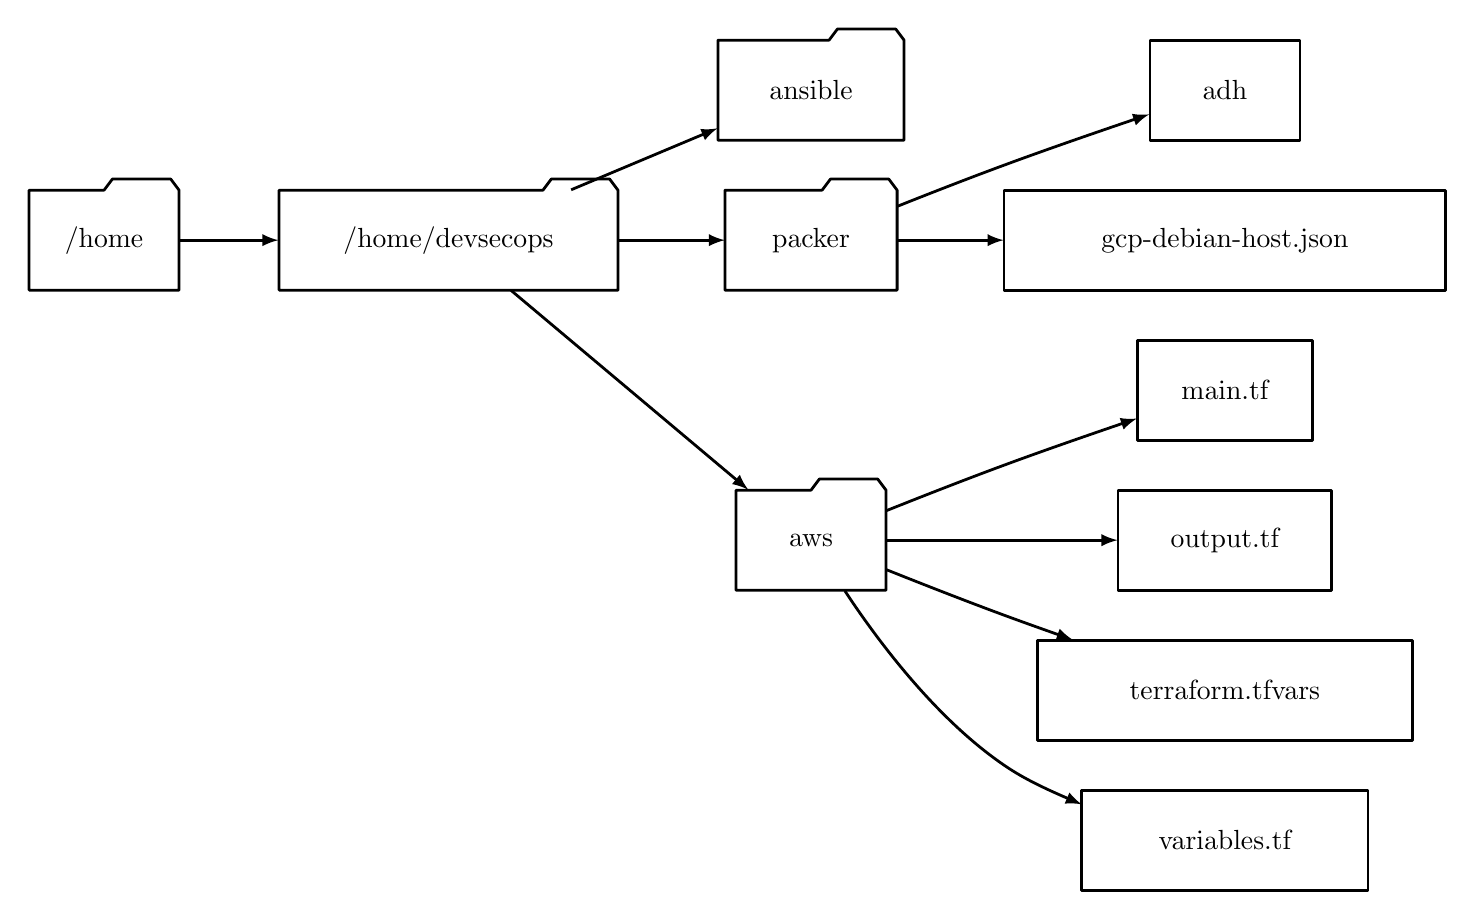
\begin{tikzpicture}[>=latex,line join=bevel,]
  \pgfsetlinewidth{1bp}
%%
\pgfsetcolor{black}
  % Edge: home -> devsecops
  \draw [->] (54.172bp,234.0bp) .. controls (61.803bp,234.0bp) and (70.527bp,234.0bp)  .. (89.778bp,234.0bp);
  % Edge: devsecops -> ansible
  \draw [->] (195.15bp,252.13bp) .. controls (209.13bp,258.01bp) and (224.61bp,264.51bp)  .. (247.83bp,274.27bp);
  % Edge: devsecops -> packer
  \draw [->] (212.11bp,234.0bp) .. controls (221.69bp,234.0bp) and (231.39bp,234.0bp)  .. (250.5bp,234.0bp);
  % Edge: devsecops -> aws
  \draw [->] (173.51bp,215.92bp) .. controls (194.73bp,198.09bp) and (227.33bp,170.69bp)  .. (258.92bp,144.14bp);
  % Edge: packer -> adh
  \draw [->] (312.74bp,246.25bp) .. controls (324.62bp,250.98bp) and (338.41bp,256.36bp)  .. (351.0bp,261.0bp) .. controls (364.79bp,266.09bp) and (380.06bp,271.41bp)  .. (403.23bp,279.29bp);
  % Edge: packer -> gdh
  \draw [->] (312.6bp,234.0bp) .. controls (321.04bp,234.0bp) and (330.68bp,234.0bp)  .. (350.84bp,234.0bp);
  % Edge: aws -> main
  \draw [->] (308.74bp,136.66bp) .. controls (321.45bp,141.74bp) and (336.97bp,147.82bp)  .. (351.0bp,153.0bp) .. controls (363.38bp,157.57bp) and (376.94bp,162.32bp)  .. (398.82bp,169.8bp);
  % Edge: aws -> out
  \draw [->] (308.78bp,126.0bp) .. controls (329.01bp,126.0bp) and (357.52bp,126.0bp)  .. (391.85bp,126.0bp);
  % Edge: aws -> tfvars
  \draw [->] (308.74bp,115.34bp) .. controls (321.45bp,110.26bp) and (336.97bp,104.18bp)  .. (351.0bp,99.0bp) .. controls (355.86bp,97.207bp) and (360.91bp,95.385bp)  .. (375.76bp,90.131bp);
  % Edge: aws -> var
  \draw [->] (293.69bp,107.73bp) .. controls (305.74bp,89.464bp) and (326.53bp,61.743bp)  .. (351.0bp,45.0bp) .. controls (356.67bp,41.118bp) and (362.96bp,37.745bp)  .. (379.0bp,30.869bp);
  % Node: home
\begin{scope}
  \definecolor{strokecol}{rgb}{0.0,0.0,0.0};
  \pgfsetstrokecolor{strokecol}
  \draw (54.0bp,252.0bp) -- (51.0bp,256.0bp) -- (30.0bp,256.0bp) -- (27.0bp,252.0bp) -- (0.0bp,252.0bp) -- (0.0bp,216.0bp) -- (54.0bp,216.0bp) -- cycle;
  \draw (27.0bp,234.0bp) node {/home};
\end{scope}
  % Node: devsecops
\begin{scope}
  \definecolor{strokecol}{rgb}{0.0,0.0,0.0};
  \pgfsetstrokecolor{strokecol}
  \draw (212.0bp,252.0bp) -- (209.0bp,256.0bp) -- (188.0bp,256.0bp) -- (185.0bp,252.0bp) -- (90.0bp,252.0bp) -- (90.0bp,216.0bp) -- (212.0bp,216.0bp) -- cycle;
  \draw (151.0bp,234.0bp) node {/home/devsecops};
\end{scope}
  % Node: ansible
\begin{scope}
  \definecolor{strokecol}{rgb}{0.0,0.0,0.0};
  \pgfsetstrokecolor{strokecol}
  \draw (315.0bp,306.0bp) -- (312.0bp,310.0bp) -- (291.0bp,310.0bp) -- (288.0bp,306.0bp) -- (248.0bp,306.0bp) -- (248.0bp,270.0bp) -- (315.0bp,270.0bp) -- cycle;
  \draw (281.5bp,288.0bp) node {ansible};
\end{scope}
  % Node: packer
\begin{scope}
  \definecolor{strokecol}{rgb}{0.0,0.0,0.0};
  \pgfsetstrokecolor{strokecol}
  \draw (312.5bp,252.0bp) -- (309.5bp,256.0bp) -- (288.5bp,256.0bp) -- (285.5bp,252.0bp) -- (250.5bp,252.0bp) -- (250.5bp,216.0bp) -- (312.5bp,216.0bp) -- cycle;
  \draw (281.5bp,234.0bp) node {packer};
\end{scope}
  % Node: aws
\begin{scope}
  \definecolor{strokecol}{rgb}{0.0,0.0,0.0};
  \pgfsetstrokecolor{strokecol}
  \draw (308.5bp,144.0bp) -- (305.5bp,148.0bp) -- (284.5bp,148.0bp) -- (281.5bp,144.0bp) -- (254.5bp,144.0bp) -- (254.5bp,108.0bp) -- (308.5bp,108.0bp) -- cycle;
  \draw (281.5bp,126.0bp) node {aws};
\end{scope}
  % Node: adh
\begin{scope}
  \definecolor{strokecol}{rgb}{0.0,0.0,0.0};
  \pgfsetstrokecolor{strokecol}
  \draw (457.5bp,306.0bp) -- (403.5bp,306.0bp) -- (403.5bp,270.0bp) -- (457.5bp,270.0bp) -- cycle;
  \draw (430.5bp,288.0bp) node {adh};
\end{scope}
  % Node: gdh
\begin{scope}
  \definecolor{strokecol}{rgb}{0.0,0.0,0.0};
  \pgfsetstrokecolor{strokecol}
  \draw (510.0bp,252.0bp) -- (351.0bp,252.0bp) -- (351.0bp,216.0bp) -- (510.0bp,216.0bp) -- cycle;
  \draw (430.5bp,234.0bp) node {gcp-debian-host.json};
\end{scope}
  % Node: main
\begin{scope}
  \definecolor{strokecol}{rgb}{0.0,0.0,0.0};
  \pgfsetstrokecolor{strokecol}
  \draw (462.0bp,198.0bp) -- (399.0bp,198.0bp) -- (399.0bp,162.0bp) -- (462.0bp,162.0bp) -- cycle;
  \draw (430.5bp,180.0bp) node {main.tf};
\end{scope}
  % Node: out
\begin{scope}
  \definecolor{strokecol}{rgb}{0.0,0.0,0.0};
  \pgfsetstrokecolor{strokecol}
  \draw (469.0bp,144.0bp) -- (392.0bp,144.0bp) -- (392.0bp,108.0bp) -- (469.0bp,108.0bp) -- cycle;
  \draw (430.5bp,126.0bp) node {output.tf};
\end{scope}
  % Node: tfvars
\begin{scope}
  \definecolor{strokecol}{rgb}{0.0,0.0,0.0};
  \pgfsetstrokecolor{strokecol}
  \draw (498.0bp,90.0bp) -- (363.0bp,90.0bp) -- (363.0bp,54.0bp) -- (498.0bp,54.0bp) -- cycle;
  \draw (430.5bp,72.0bp) node {terraform.tfvars};
\end{scope}
  % Node: var
\begin{scope}
  \definecolor{strokecol}{rgb}{0.0,0.0,0.0};
  \pgfsetstrokecolor{strokecol}
  \draw (482.0bp,36.0bp) -- (379.0bp,36.0bp) -- (379.0bp,0.0bp) -- (482.0bp,0.0bp) -- cycle;
  \draw (430.5bp,18.0bp) node {variables.tf};
\end{scope}
%
\end{tikzpicture}


	\caption{Tool related files and folders.}
\end{figure}
